\section{Resultados}

\subsection{Análisis del método propuesto}
\begin{frame}[allowframebreaks,fragile]
	\frametitle{Análisis del método propuesto}

	\textbf{Metodología utilizada}
	\bigskip

	\begin{itemize}[<*>]
		\item Se comparan distintas ejecuciones del método EQuAL.
		\item Se varia el tamaño de muestra en particular: 100, 500, 1000, 1500 y 2000 pares de preguntas.
		\item Por cada uno de los tamaños de muestra se varia el número de clusters \(k\) distinto: 5, 10, 15, 20, 25, 30, 35, 40, 45 y 50.
	\end{itemize}

	\framebreak

	\begin{table}[h!]
		\scriptsize
		\resizebox{\columnwidth}{!}{%
		\begin{tabularx}{\textwidth}{XXXXXXXX}
			\toprule
			\textbf{k / Tam. muestra} &
			\textbf{100} &
			\textbf{500} &
			\textbf{1000} &
			\textbf{1500} &
			\textbf{2000} &
			\textbf{Media} &
			\textbf{Varianza} \\ \midrule
			\textbf{5}  & 0.322 & 0.3366 & 0.3463 & 0.3486 & 0.3407 & 0.33884                         & 0.0004429                         \\
			\textbf{10} & 0.318 & 0.3254 & 0.3406 & 0.3395 & 0.3389 & 0.33248                         & \cellcolor[HTML]{D9EAD3}0.0004162 \\
			\textbf{15} & 0.314 & 0.325  & 0.3419 & 0.341  & 0.3354 & 0.33146                         & 0.0005621                       \\
			\textbf{20} & 0.318 & 0.3192 & 0.3393 & 0.3424 & 0.3375 & 0.33128                         & 0.0005489                        \\
			\textbf{25} & 0.309 & 0.3226 & 0.3378 & 0.3397 & 0.3354 & 0.3289                          & 0.0006738                           \\
			\textbf{30} & 0.304 & 0.3218 & 0.3364 & 0.3384 & 0.3353 & 0.32718                         & 0.0008430                        \\
			\textbf{35} & 0.307 & 0.3188 & 0.3366 & 0.3364 & 0.3315 & 0.32606                         & 0.0006635                       \\
			\textbf{40} & 0.309 & 0.317  & 0.3397 & 0.3384 & 0.3296 & 0.32674                         & 0.0007216                      \\
			\textbf{45} & 0.311 & 0.3162 & 0.3361 & 0.335  & 0.3317 & 0.326                           & 0.000536                      \\
			\textbf{50} & 0.308 & 0.314  & 0.3324 & 0.3293 & 0.3306 & \cellcolor[HTML]{D9EAD3}0.32286 & 0.0004917                         \\
			\midrule
			\textbf{Media} &
			\cellcolor[HTML]{D9EAD3}0.312 &
			0.32166 &
			0.33871 &
			0.33887 &
			0.33466 &
			\\
			\textbf{Varianza} &
			0.0003 &
			0.0003736 &
			0.0001299 &
			0.0002258 &
			\cellcolor[HTML]{D9EAD3}0.0001248 &
			\\
			\bottomrule
		\end{tabularx}
		}
		\label{tab:analisis-error-vs-k}
	\end{table}

	\framebreak

	\begin{filecontents*}{erroresktamanomuestra1.csv}
		100,0.322,0.318,0.314,0.318,0.309,0.304,0.307,0.309,0.311,0.308
		500,0.3366,0.3254,0.325,0.3192,0.3226,0.3218,0.3188,0.317,0.3162,0.314
		1000,0.3463,0.3406,0.3419,0.3393,0.3378,0.3364,0.3366,0.3397,0.3361,0.3324
		1500,0.3486,0.3395,0.341,0.3424,0.3397,0.3384,0.3364,0.3384,0.335,0.3293
		2000,0.3407,0.3389,0.3354,0.3375,0.3354,0.3353,0.3315,0.3296,0.3317,0.3306
	\end{filecontents*}

	Errores de los valores de \(k\) para los distintos tamaños de muestra:
	\begin{figure}
		\centering
		\scriptsize
		\resizebox{0.7\textwidth}{!}{%
			\begin{tikzpicture}
				\begin{axis}[
					xlabel={Tamaños de muestra},
					ylabel={Error},
					xmin=100, xmax=2000,
					ymin=0.30, ymax=0.36,
					xtick={100,500,1000,1500,2000},
					ytick={0.30,0.31,...,0.36},
					legend pos=north west,
					ymajorgrids=true,
					grid style=dashed,
					clip=false,
					]

					\addplot table [mark=square,x index=0, y index=1, col sep=comma] {erroresktamanomuestra1.csv};
					\label{k5}
					\addplot table [mark=square,x index=0, y index=2, col sep=comma] {erroresktamanomuestra1.csv};
					\label{k10}
					\addplot table [mark=square,x index=0, y index=3, col sep=comma] {erroresktamanomuestra1.csv};
					\label{k15}
					\addplot table [mark=square,x index=0, y index=4, col sep=comma] {erroresktamanomuestra1.csv};
					\label{k20}
					\addplot table [mark=square,x index=0, y index=5, col sep=comma] {erroresktamanomuestra1.csv};
					\label{k25}
					\addplot table [mark=square,x index=0, y index=5, col sep=comma] {erroresktamanomuestra1.csv};
					\label{k30}
					\addplot table [mark=square,x index=0, y index=7, col sep=comma] {erroresktamanomuestra1.csv};
					\label{k35}
					\addplot table [mark=square,x index=0, y index=8, col sep=comma] {erroresktamanomuestra1.csv};
					\label{k40}
					\addplot table [mark=square,x index=0, y index=9, col sep=comma] {erroresktamanomuestra1.csv};
					\label{k45}
					\addplot table [mark=square,x index=0, y index=10, col sep=comma] {erroresktamanomuestra1.csv};
					\label{k50}
				\end{axis}

				% Primer cuadro de leyendas.
				\node [draw,fill=white] at (rel axis cs: 0.55,0.2) {\scriptsize\shortstack[l]{
						\ref{k5} $k = 5$ \\
						\ref{k10} $k = 10$ \\
						\ref{k15} $k = 15$ \\
						\ref{k20} $k = 20$ \\
						\ref{k25} $k = 25$}};

				% Segundo cuadro de leyendas.
				\node [draw,fill=white] at (rel axis cs: 0.83,0.2) {\scriptsize\shortstack[l]{
						\ref{k30} $k = 30$ \\
						\ref{k35} $k = 35$ \\
						\ref{k40} $k = 40$ \\
						\ref{k45} $k = 45$ \\
						\ref{k50} $k = 50$}};
			\end{tikzpicture}
		}
		\label{fig:errores-k-tamanos-muestra}
	\end{figure}

	\begin{filecontents*}{errorestamanomuestrak1.csv}
		5,0.322,0.3366,0.3463,0.3486,0.3407
		10,0.318,0.3254,0.3406,0.3395,0.3389
		15,0.314,0.325,0.3419,0.341,0.3354
		20,0.318,0.3192,0.3393,0.3424,0.3375
		25,0.309,0.3226,0.3378,0.3397,0.3354
		30,0.304,0.3218,0.3364,0.3384,0.3353
		35,0.307,0.3188,0.3366,0.3364,0.3315
		40,0.309,0.317,0.3397,0.3384,0.3296
		45,0.311,0.3162,0.3361,0.335,0.3317
		50,0.308,0.314,0.3324,0.3293,0.3306
	\end{filecontents*}

	Errores de los distintos tamaños de muestra para los valores de  \(k\).
	\begin{figure}[h!]
		\centering
		\scriptsize
		\resizebox{0.7\textwidth}{!}{%
			\begin{tikzpicture}
				\begin{axis}[
					xlabel={Valores de k},
					ylabel={Error},
					xmin=5, xmax=50,
					ymin=0.30, ymax=0.37,
					xtick={5,10,...,50},
					ytick={0.30,0.31,...,0.37},
					legend pos=north west,
					ymajorgrids=true,
					grid style=dashed,
					]

					\addplot table [mark=square,x index=0, y index=1, col sep=comma] {errorestamanomuestrak1.csv};
					\label{t100}
					\addplot table [mark=square,x index=0, y index=2, col sep=comma] {errorestamanomuestrak1.csv};
					\label{t500}
					\addplot table [mark=square,x index=0, y index=3, col sep=comma] {errorestamanomuestrak1.csv};
					\label{t1000}
					\addplot table [mark=square,x index=0, y index=4, col sep=comma] {errorestamanomuestrak1.csv};
					\label{t1500}
					\addplot table [mark=square,x index=0, y index=5, col sep=comma] {errorestamanomuestrak1.csv};
					\label{t2000}
				\end{axis}

				% Cuadro de leyendas.
				\node [draw,fill=white] at (rel axis cs: 0.85,0.8) {\scriptsize\shortstack[l]{
						\ref{t100} $100$ \\
						\ref{t500} $500$ \\
						\ref{t1000} $1000$ \\
						\ref{t1500} $1500$ \\
						\ref{t2000} $2000$}};
			\end{tikzpicture}
		}
		\label{fig:errores-tamanos-muestra-k}
	\end{figure}
\end{frame}

\subsection{Análisis del método propuesto y algoritmos del estado del arte}
\begin{frame}[allowframebreaks,fragile]
	\frametitle{Análisis del método propuesto y algoritmos del estado del arte}
	\textbf{Metodología utilizada}
	\bigskip

	\begin{itemize}[<*>]
		\item Se realizaron 10 ejecuciones de una muestra aleatoria para cada uno de los algoritmos del estado del arte.
		\item Se varia el tamaño de muestra en particular: 100, 500, 1000, 1500 y 2000 pares de preguntas.
		\item Por cada uno de los tamaños de muestra se varia el número de clusters \(k\) distinto: 5, 10, 15, 20, 25, 30, 35, 40, 45 y 50.
	\end{itemize}

	\framebreak

	Error en los algoritmos del estado del arte vs. método EQuAL por tamaño de muestra, media y varianza.
	\begin{table}[h!]
		\scriptsize
		\begin{tabularx}{\textwidth}{cccccccc}
			\toprule
			& \textbf{100} & \textbf{500} & \textbf{1000} & \textbf{1500} & \textbf{2000} & \textbf{Media} & \textbf{Varianza} \\
			\midrule
			\textbf{bow}      & 0.296 & 0.3122 & 0.3149 & 0.3202667 & 0.31475 & \cellcolor[HTML]{D9EAD3}0.3116233 & 0.0003396                          \\
			\textbf{ft}       & 0.334 & 0.3282 & 0.3275 & 0.3320667 & 0.33445 & 0.3312433                         & \cellcolor[HTML]{D9EAD3}0.0000418 \\
			\textbf{w2v}      & 0.317 & 0.3246 & 0.3169 & 0.3231333 & 0.32335 & 0.3209967                         & 0.0000558                         \\
			\textbf{gtfidf}   & 0.311 & 0.3218 & 0.3252 & 0.3322       & 0.33025 & 0.32409                              & 0.0002815                              \\
			\textbf{sem}      & 0.301 & 0.3176 & 0.3162 & 0.3338       & 0.3249  & 0.3187                               & 0.0005872                                \\
			\textbf{EQuAL} & 0.308 & 0.314  & 0.3324 & 0.3293       & 0.3306  & 0.32286                              & 0.0004917                              \\
			\bottomrule
		\end{tabularx}
		\label{tab:error-arte-equal}
	\end{table}

	\framebreak

	\begin{filecontents*}{ensamble-vs-medidas-1.csv}
		100,0.296,0.334,0.317,0.311,0.301,0.304
		500,0.3122,0.3282,0.3246,0.3218,0.3176,0.314
		1000,0.3149,0.3275,0.3169,0.3252,0.3162,0.3324
		1500,0.3202666667,0.3320666667,0.3231333333,0.3322,0.3338,0.3293
		2000,0.31475,0.33445,0.32335,0.33025,0.3249,0.3306
	\end{filecontents*}

	\footnotesize
	Errores de los tamaños de muestra para el método EQuAL y los algoritmos del estado del arte.
	\begin{figure}[h!]
		\centering
		\scriptsize
		\resizebox{0.6\textwidth}{!}{%
			\begin{tikzpicture}
				\begin{axis}[
					xlabel={Tamaños de muestra},
					ylabel={Error},
					xmin=100, xmax=2000,
					ymin=0.28, ymax=0.35,
					xtick={100,500,1000,1500,2000},
					ytick={0.28,0.29,...,0.35},
					legend pos=north west,
					ymajorgrids=true,
					grid style=dashed,
					]

					\addplot+ [line width=2pt] table [mark=none,x index=0, y index=6, col sep=comma] {ensamble-vs-medidas-1.csv};
					\label{EQuAL}
					\addplot table [mark=square,x index=0, y index=1, col sep=comma] {ensamble-vs-medidas-1.csv};
					\label{bow}
					\addplot table [mark=square,x index=0, y index=2, col sep=comma] {ensamble-vs-medidas-1.csv};
					\label{ft}
					\addplot table [mark=square,x index=0, y index=3, col sep=comma] {ensamble-vs-medidas-1.csv};
					\label{w2v}
					\addplot table [mark=square,x index=0, y index=4, col sep=comma] {ensamble-vs-medidas-1.csv};
					\label{tfidf}
					\addplot table [mark=square,x index=0, y index=5, col sep=comma] {ensamble-vs-medidas-1.csv};
					\label{sem}
				\end{axis}

				% Cuadro de leyendas.
				\node [draw,fill=white] at (rel axis cs: 0.82,0.2) {\scriptsize\shortstack[l]{
						\ref{bow} $bow$ \\
						\ref{ft} $ft$ \\
						\ref{w2v} $w2v$ \\
						\ref{tfidf} $tfidf$ \\
						\ref{sem} $sem$ \\
						\ref{EQuAL} $EQuAL$}};
			\end{tikzpicture}
		}
		\label{fig:ensamble-vs-medidas}
	\end{figure}

\end{frame}

\subsection{Otras observaciones de interés}
\begin{frame}[allowframebreaks,fragile]
	\frametitle{Otras observaciones de interés}
	\textbf{Análisis de varianza del método propuesto.}
	\bigskip

	Se denomina \(\mu_0\) a la esperanza de los errores del método EQuAL y se denominan \(\mu_i, i = 1,..., 5\) a las esperanzas de los errores de los métodos, TF, TF-IDF, FastText, Word2Vec y Semantic Distance, respectivamente. Se plantean las siguientes hipótesis:
	\bigskip
	\begin{itemize}[<*>]
		\item \textbf{\(H_0\)}: \(\mu_0 - \mu_i = 0, i = 1,..., 5\).
		\item \textbf{\(H_1\)}: \(\mu_0 - \mu_i \neq 0, i = 1,..., 5\).
	\end{itemize}

	\framebreak

	\footnotesize
	Tamaño de muestra de 100 pares de preguntas.
	\begin{figure}[!htbp]
		\centering
		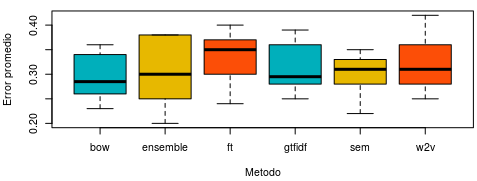
\includegraphics[width=0.7\linewidth]{../10_resultados/imagenes/anova_100}
		\label{fig:anova100-1}
	\end{figure}

	\begin{itemize}[<*>]
		\item En todos los casos, los intervalos de confianza incluyen al valor 0 y \(p{-}adj > \alpha\).
		\item El método EQuAL posee una media de error que no posee diferencias significativas a todos los métodos.
	\end{itemize}

	\framebreak

	Tamaño de muestra de 500 pares de preguntas.
	\begin{figure}[!htbp]
		\centering
		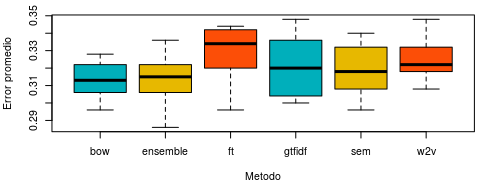
\includegraphics[width=0.7\linewidth]{../10_resultados/imagenes/anova_500}
		\label{fig:anova500-1}
	\end{figure}

	\begin{itemize}[<*>]
		\item En todos los casos, los intervalos de confianza incluyen al valor 0 y \(p{-}adj > \alpha\).
		\item El método EQuAL posee una media de error que no posee diferencias significativas a todos los métodos.
	\end{itemize}

	\framebreak

	Tamaño de muestra de 1000 pares de preguntas.
	\begin{figure}[!htbp]
		\centering
		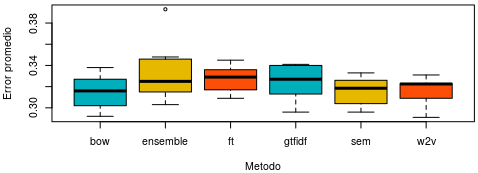
\includegraphics[width=0.7\linewidth]{../10_resultados/imagenes/anova_1000}
		\label{fig:anova1000-1}
	\end{figure}

	\begin{itemize}[<*>]
		\item En todos los casos, los intervalos de confianza incluyen al valor 0 y \(p{-}adj > \alpha\).
		\item El método EQuAL posee una media de error que no posee diferencias significativas a todos los métodos.
	\end{itemize}

	\framebreak

	Tamaño de muestra de 1500 pares de preguntas.
	\begin{figure}[!htbp]
		\centering
		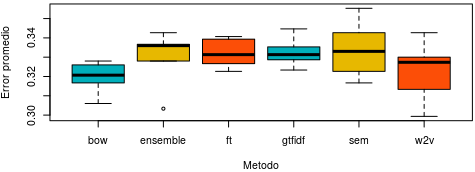
\includegraphics[width=0.7\linewidth]{../10_resultados/imagenes/anova_1500}
		\label{fig:anova1500-1}
	\end{figure}

	\begin{itemize}[<*>]
		\item En todos los casos, los intervalos de confianza incluyen al valor 0 y \(p{-}adj > \alpha\).
		\item El método EQuAL posee una media de error que no posee diferencias significativas a todos los métodos.
	\end{itemize}

	\framebreak

	Tamaño de muestra de 2000 pares de preguntas.
	\begin{figure}[!htbp]
		\centering
		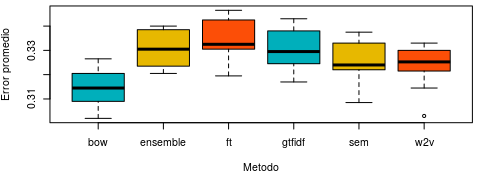
\includegraphics[width=0.7\linewidth]{../10_resultados/imagenes/anova_2000}
		\label{fig:anova2000-1}
	\end{figure}

	\begin{itemize}[<*>]
		\item El intervalo de confianza contra el método bow no incluye al cero, ya que este método tuvo muy buenos indicadores en este tamaño de muestra.
		\item En el resto de los casos, los intervalos de confianza incluyen al valor 0 y \(p{-}adj > \alpha\).
	\end{itemize}

	\framebreak

	\normalsize
	\textbf{Resumen de resultados del análisis de varianza}
	\bigskip
	\begin{itemize}[<*>]
		\item Se realizaron 25 intervalos de confianza, y en solo uno el método EQuAL se obtuvo una media de error más alta, ya que el método bow fue significativamente mejor al resto.
		\item El método EQuAL tiene un buen comportamiento en cuanto a medias de error a lo largo de todos los tamaños de muestra.
		\item Las esperanzas de error no tienen diferencias significativas con los métodos del estado del arte.
		\item Se puede concluir que el método EQuAL es apto para su implementación en RS.
	\end{itemize}

	\framebreak

	\textbf{Otras observaciones}
	\bigskip
	\begin{itemize}[<*>]
		\item El agregado de variabilidad de datos puede ser influyente en tamaños de muestra pequeños.
		\item El método EQuAL es dependiente a los métodos subyacentes.
		\item Debido a la naturaleza del conjunto de datos utilizado, no es posible identificar fácilmente cuál es la forma de los clusters en cuestión, y verificar si el método EQuAL se adapta perfectamente al conjunto de datos.
	\end{itemize}

\end{frame}

\subsection{Análisis de desempeño}
\begin{frame}[allowframebreaks, fragile]
	\frametitle{Análisis de desempeño}
	Se realizó un \textbf{análisis de desempeño} con las siguientes características:
	\bigskip
	\begin{itemize}[<*>]
		\item Cluster Hadoop en localhost.
		\item Tamaños de muestra 100, 500 y 1000 pares de preguntas.
		\item En cada una de las ejecuciones, utilizan dos técnicas de similaridad (TF y TFIDF), para luego ensamblarlas.
		\item Cantidad de núcleos CPU asignados: 1, 2, 4, 8 y 12.
	\end{itemize}

	\framebreak

	\begin{filecontents*}{performance-100-1.csv}
		1,62.9900532,15.978281,88.5538612
		2,46.080726,10.388303,64.830457
		4,33.073601,6.872383,47.60667
		8,31.275526,6.30869,45.023509
		12,32.336151,5.69793,44.428017
	\end{filecontents*}

	\footnotesize
	Tamaño de muestra de 100 pares de preguntas y distintos núcleos de CPU.
	\begin{figure}[h!]
		\centering
		\scriptsize
		\resizebox{0.7\textwidth}{!}{%
			\begin{tikzpicture}
				\begin{axis}[
					xlabel={Número de núcleos de CPU},
					ylabel={Tiempo (Seg.)},
					xmin=0, xmax=13,
					ymin=0, ymax=100,
					xtick={1,2,4,8,12},
					ytick={0,10,...,100},
					legend pos=north west,
					ymajorgrids=true,
					grid style=dashed,
					]

					\addplot table [mark=square,x index=0, y index=1, col sep=comma] {performance-100-1.csv};
					\label{similaridad100}
					\addplot table [mark=square,x index=0, y index=2, col sep=comma] {performance-100-1.csv};
					\label{ensamble100}
					\addplot table [mark=square,x index=0, y index=3, col sep=comma] {performance-100-1.csv};
					\label{total100}
				\end{axis}

				% Cuadro de leyendas.
				\node [draw,fill=white] at (rel axis cs: 0.66,0.85) {\scriptsize\shortstack[l]{
						\ref{similaridad100} Cálculo de Similaridad \\
						\ref{ensamble100} Ensamble de Clustering \\
						\ref{total100} Total}};
			\end{tikzpicture}
		}
		\label{fig:performance100}
	\end{figure}

	\framebreak

	\begin{filecontents*}{performance-500-1.csv}
		1,763.888817,40.430,828.022
		2,576.668802,25.684,624.102
		4,402.376359,21.511,446.984
		8,324.825807,18.017,363.617
		12,328.300206,15.737,362.982
	\end{filecontents*}

	Tamaño de muestra de 500 pares de preguntas y distintos núcleos de CPU.
	\begin{figure}[h!]
		\centering
		\scriptsize
		\resizebox{0.7\textwidth}{!}{%
			\begin{tikzpicture}
				\begin{axis}[
					xlabel={Número de núcleos de CPU},
					ylabel={Tiempo (Seg.)},
					xmin=0, xmax=13,
					ymin=0, ymax=1000,
					xtick={1,2,4,8,12},
					ytick={0,100,...,1000},
					legend pos=north west,
					ymajorgrids=true,
					grid style=dashed,
					]

					\addplot table [mark=square,x index=0, y index=1, col sep=comma] {performance-500-1.csv};
					\label{similaridad500}
					\addplot table [mark=square,x index=0, y index=2, col sep=comma] {performance-500-1.csv};
					\label{ensamble500}
					\addplot table [mark=square,x index=0, y index=3, col sep=comma] {performance-500-1.csv};
					\label{total500}
				\end{axis}

				% Cuadro de leyendas.
				\node [draw,fill=white] at (rel axis cs: 0.66,0.85) {\scriptsize\shortstack[l]{
						\ref{similaridad500} Cálculo de Similaridad \\
						\ref{ensamble500} Ensamble de Clustering \\
						\ref{total500} Total}};
			\end{tikzpicture}
		}
		\label{fig:performance500}
	\end{figure}

	\framebreak

	\begin{filecontents*}{performance-1000-1.csv}
		1,2950.810,95.886,3106.846134
		2,2073.179,58.053,2199.751862
		4,1423.896,47.732525,1530.309932
		8,1176.593,43.265526,1282.804328
		12,1253.434,43.699182,1370.473092
	\end{filecontents*}

	Tamaño de muestra de 1000 pares de preguntas y distintos núcleos de CPU.
	\begin{figure}[h!]
		\centering
		\scriptsize
		\resizebox{0.7\textwidth}{!}{%
			\begin{tikzpicture}
				\begin{axis}[
					xlabel={Número de núcleos de CPU},
					ylabel={Tiempo (Seg.)},
					xmin=0, xmax=13,
					ymin=0, ymax=3500,
					xtick={1,2,4,8,12},
					ytick={0,500,...,3500},
					legend pos=north west,
					ymajorgrids=true,
					grid style=dashed,
					]

					\addplot table [mark=square,x index=0, y index=1, col sep=comma] {performance-1000-1.csv};
					\label{similaridad1000}
					\addplot table [mark=square,x index=0, y index=2, col sep=comma] {performance-1000-1.csv};
					\label{ensamble1000}
					\addplot table [mark=square,x index=0, y index=3, col sep=comma] {performance-1000-1.csv};
					\label{total1000}
				\end{axis}

				% Cuadro de leyendas.
				\node [draw,fill=white] at (rel axis cs: 0.66,0.85) {\scriptsize\shortstack[l]{
						\ref{similaridad1000} Cálculo de Similaridad \\
						\ref{ensamble1000} Ensamble de Clustering \\
						\ref{total1000} Total}};
			\end{tikzpicture}
		}
		\label{fig:performance1000}
	\end{figure}

\end{frame}

\subsection{Resumen de resultados}
\begin{frame}
	\frametitle{Resumen de resultados}
	\textbf{Resumen de resultados}
	\bigskip
	\begin{itemize}
		\item El método EQuAL tuvo buen rendimiento con tamaños pequeños de muestras y con un alto número de clusters.
		\item Comparando el método EQuAL con los algoritmos del estado del arte, se concluye que posee indicadores aptos para su aplicación en RS, en cuanto a medias de error y varianza.
		\item Es altamente probable que el método EQuAL arroje buenos resultados si los algoritmos subyacentes también lo hacen, y viceversa.
		\item Es posible adaptar el método al conjunto de datos y elegir los algoritmos subyacentes adecuados.
		\item Se desarrolló una arquitectura de software con enfoque Big Data que realiza los cálculos de similaridad y procesamiento del ensamble de clustering de manera escalable y adaptable.
	\end{itemize}
\end{frame}